\documentclass[aspectratio=169]{beamer}

\usepackage{graphicx}
\usepackage{booktabs}
\usepackage{subfigure}
\usepackage[bookmarks=true]{hyperref}
\usepackage{blkarray}
\usefonttheme{serif}

\mode<presentation> {
    \usetheme{Madrid}
    \usecolortheme{rose}

    \AtBeginSection[]{
        \begin{frame}{Overview}
            \tableofcontents[sectionstyle=show/shaded,subsectionstyle=show/shaded/hide]
        \end{frame}
    }

}

\title[Scaling Laws]{
    Exploring Scaling Laws in LLM Pretraining
}

\author{Zibo Ren, Runlin Chen}
\institute[PKU]
{
    Peking University \\
    \medskip
    \texttt{\{2200010626,2200010848\}@stu.pku.edu.cn}
}
\date{\today}

\begin{document}

    \begin{frame}
        \titlepage
    \end{frame}

    \begin{frame}
        \frametitle{Overview}
        \tableofcontents
    \end{frame}


    \section{Scaling Laws}\label{sec:scalinglaws}

    \subsection{Chinchilla Scaling Law}\label{subsec:chinchilla}
    \begin{frame}
        \frametitle{Chinchilla Scaling Law}
        \begin{block}{Chinchilla Scaling Law}
            \begin{equation}
                \label{eq:chinchilla}
                \begin{aligned}
                    L(D, N) &= L_0 + A\cdot D^{-\alpha} + B\cdot N^{-\beta} \\
                \end{aligned}
            \end{equation}
        \end{block}
        \begin{itemize}
            \item $L(D, N)$ is the final validation loss.
            \item $D$ is the amount of data.
            \item $N$ is the number of parameters.
            \item $L_0$, $A$, $B$, $\alpha$ and $\beta$ are undetermined
            positive constants.
        \end{itemize}

        It only illustrates the loss at the end of training, but not the
        loss during training.
    \end{frame}

    \subsection{Scaling Law with LR Annealing (LRA)}\label{subsec:LRA}

    \begin{frame}
        \frametitle{Scaling Law with LR Annealing}
        \begin{block}{Scaling Low Formula}
            \begin{equation}
                \label{eq:scaling_low}
                \begin{aligned}
                    L(s) &= L_0 + A\cdot S_1^{-\alpha} - C\cdot S_2 \\
                    S_1 &= \sum_{i=1}^{s} \eta_i \\
                    S_2 &= \sum_{i=1}^{s} \sum_{k=1}^{i} (\eta_{k-1} -
                    \eta_k)\cdot\lambda^{i-k}
                \end{aligned}
            \end{equation}
        \end{block}

        \begin{enumerate}
            \item $L(s)$: the loss at step $s$.
            \item $\eta_i$: the learning rate at step $i$.
            \item $\lambda$: a hyper-parameter to notate the decay factor
            in LR annealing momentum.
        \end{enumerate}
    \end{frame}

    \begin{frame}
        \frametitle{Scaling Law with LR Annealing}
        As an extension of Chinchilla scaling law, we can write the scaling law as
        \begin{equation}
            L(s) = L_0 + A\cdot S_1^{-\alpha} - f(\eta)
        \end{equation}
        The second term is an extension of the Chinchilla scaling law and
        the third term is a correction term for the learning rate decay.

        \textbf{Observation from Experiments:} there is a delay between
        learning rate
        changes and loss changes, so we write $f(\eta)$ as a form of momentum:
        \begin{equation}
            \begin{aligned}
                m_i &= \lambda m_{i-1} + (\eta_{i-1} - \eta_i) \\
                f(\eta) &= \sum_{i=1}^{s} m_i
            \end{aligned}
        \end{equation}
    \end{frame}

    \begin{frame}
        \frametitle{Defect of Scaling Law with LR Annealing}
        \begin{enumerate}
            \item If the we add some iterations with learning rate 0 to
            the end of the training, according to
            (\ref{eq:scaling_low}), the loss will still decrease dual
            to $S_1$ is not change and $S_2$ is increasing.
            \item Multiplying the entire schedule elementwise by a
            positive constant larger than 1 always decreases the predicted loss.
            If we set the learning rate to approach positive infinity
            during the first iteration and subsequently fix it at
            zero, this would theoretically yield a negative loss
            value, which clearly contradicts empirical observations.
            \item The form of $S_2$ is based on observation, but it is lack of
            theoretical support.
        \end{enumerate}
    \end{frame}

    \subsection{Multi-Power Law}\label{subsec:MPL}

    \begin{frame}
        \frametitle{Multi-Power Law}
        \begin{block}{Multi-Power Law}
            \begin{equation}
                \label{eq:multi_power_law}
                \begin{aligned}
                    &L(t) = L_0 + A\cdot (S_1(t) + S_W)^{-\alpha} - LD(t)\\
                    &\text{where} \\
                    & LD(t) = B\sum_{k=1}^{t}(\eta_{k-1}-\eta_k)\cdot
                    G(\eta_k^{-\gamma}S_k(t)), \\
                    &S_k(t) = \sum_{i=k}^{t} \eta_i, \\
                    &G(x) = 1-(Cx+1)^{-\beta}
                \end{aligned}
            \end{equation}
        \end{block}

        \begin{enumerate}
            \item $A\cdot (S_1(t) + S_W)^{-\alpha}$ is an extension of
            Chinchilla scaling law.
            \item $LD(t)$ is a correction term to account for the
            learning rate decay.
            \item Actually $G(x)$ can be any increasing function that
            maps $[0, \inf]$ to $[0, 1]$.
        \end{enumerate}
    \end{frame}

    \begin{frame}
        \frametitle{Multi-Power Law}
        \textbf{Observation:} If the sum of learning rates is identical, the
        loss at the end of training is similar, so we can write the loss
        as the following form:
        \begin{equation}
            L(t) = L_0 + A\cdot (S_1(t)-S_W)^{-\alpha} - LD(t)
        \end{equation}

        \textbf{Two-Stage Learning Rate Schedule:}
        \begin{enumerate}
            \item As $t$ increases, the difference between two learning
            rates schedulers is also increasing and eventually saturates.
            So we write $LD(T_A+x) = \tilde{B}(1-U(\eta_B x))$.
            \item According to experiments, $U(s) =
            (\tilde{C}s+1)^{-\beta}$ is a power-law form.
            \item $\tilde{B}$ is linear to the LR reduction, and $\tilde{C}$
            is a power-law of $\eta_B$.
        \end{enumerate}
        \begin{figure}
            \centering
            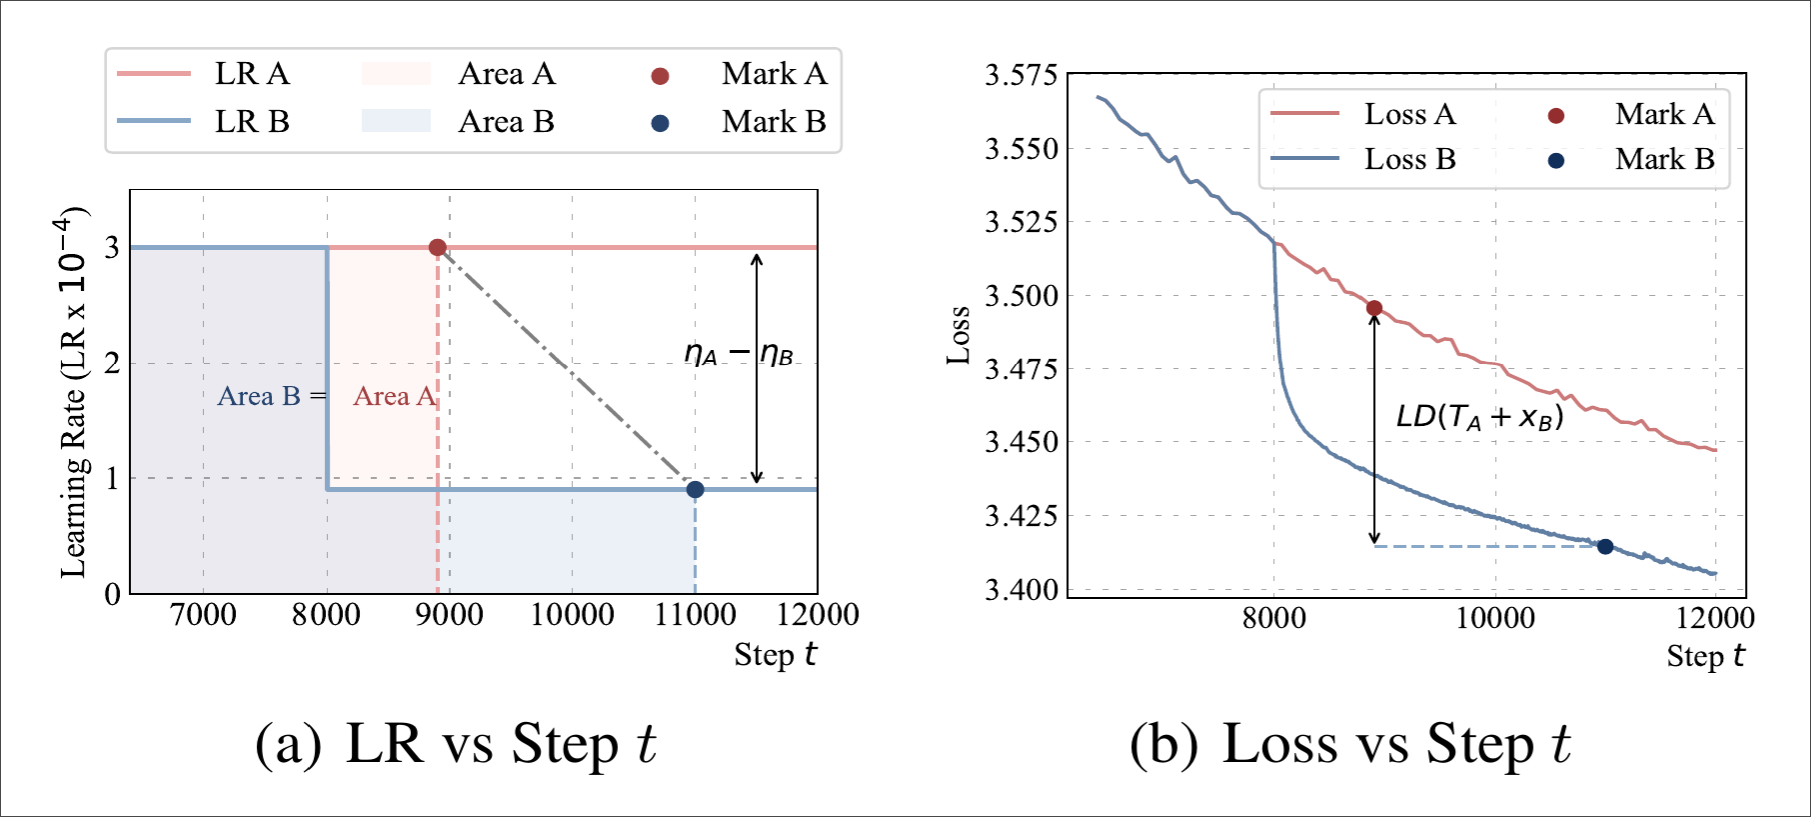
\includegraphics[width=0.4\textwidth]{fig/mpl.png}
        \end{figure}
    \end{frame}

    \begin{frame}
        \frametitle{Defect of Multi-Power Law}
        If the we add some iterations with learning rate 0
        to the training process, the loss will not change actually.
        For example, the learning rate list $[\eta_0,0,\eta_0,0]$ should
        get the same loss as $[\eta_0,\eta_0]$.
        But using MPL, we will get different loss values because
        the $G(x)$ term cannot cancel each other.
    \end{frame}


    \section{Experiments}\label{sec:experiments}

    \begin{frame}
        \frametitle{Experiments Setup}
        \begin{enumerate}
            \item We use the loss curves of a 100M GPT model trained on
            20B tokens of data.
            \item We use 3 types of learning rate schedules: "8-1-1",
            warmup-stable-decay(WSD) and cosine.
            \item The total train step is 33907, we use the first 10000
            of one learning rate schedule to fit the parameters of
            the model and test the model on the full loss curve of
            the three learning rate schedules.
            \item For both LRA and MPL, we use the SGD optimizer to fit
            the parameters.
            \item For MPL, we conducted a set of ablation experiments.The
            following methods are all
            modified from the original MPL: OPL means $LD(t)=0$, LLDL
            means $G(x)=1$ and MEL means $G(x) = 1-e^{-Cx},\gamma = 0$
            \item Our code and data are available at
            \url{https://github.com/0Ishtar0/explore-scaling-law.git}
        \end{enumerate}
    \end{frame}

    \begin{frame}
        \frametitle{Experiments Results of LRA}
        We use cosine learning rate schedule to fit the parameters
        \begin{figure}
            \centering
            \subfigure[cosine learning rate]{
                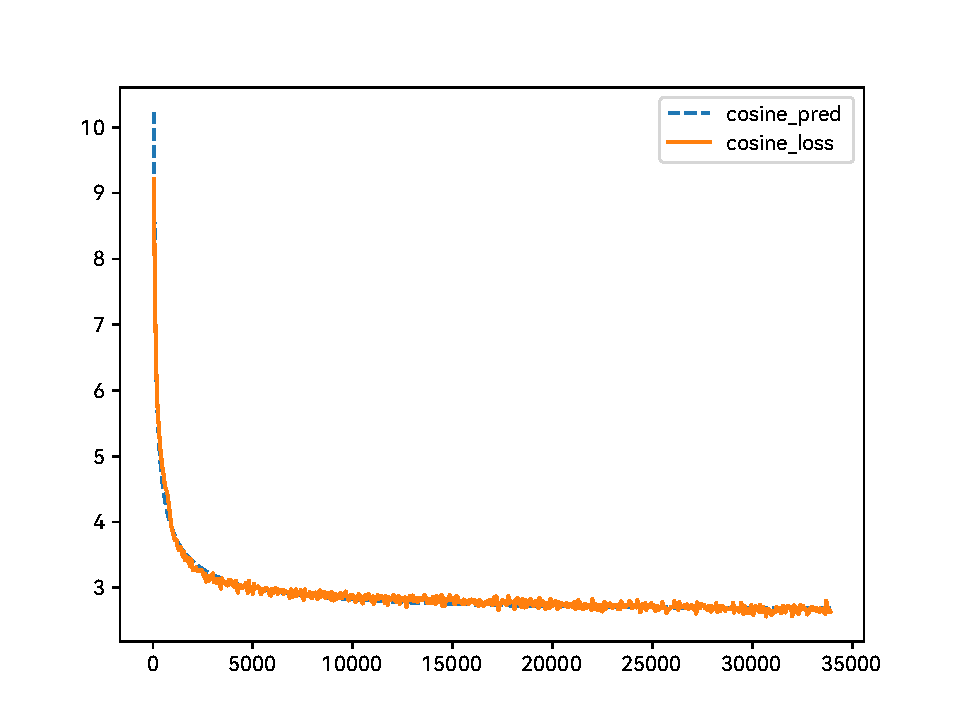
\includegraphics[width=0.3\textwidth]{fig/lra/cosine_fit.pdf}
            }
            \subfigure[8-1-1 learning rate]{
                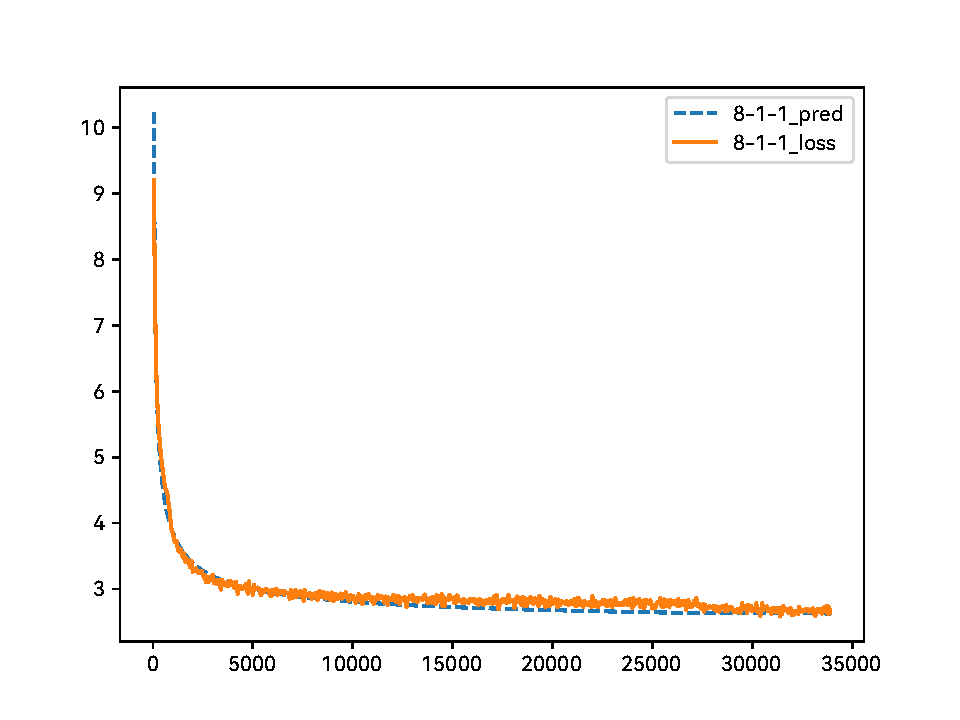
\includegraphics[width=0.3\textwidth]{fig/lra/8-1-1_fit.pdf}
            }
            \subfigure[WSD learning rate]{
                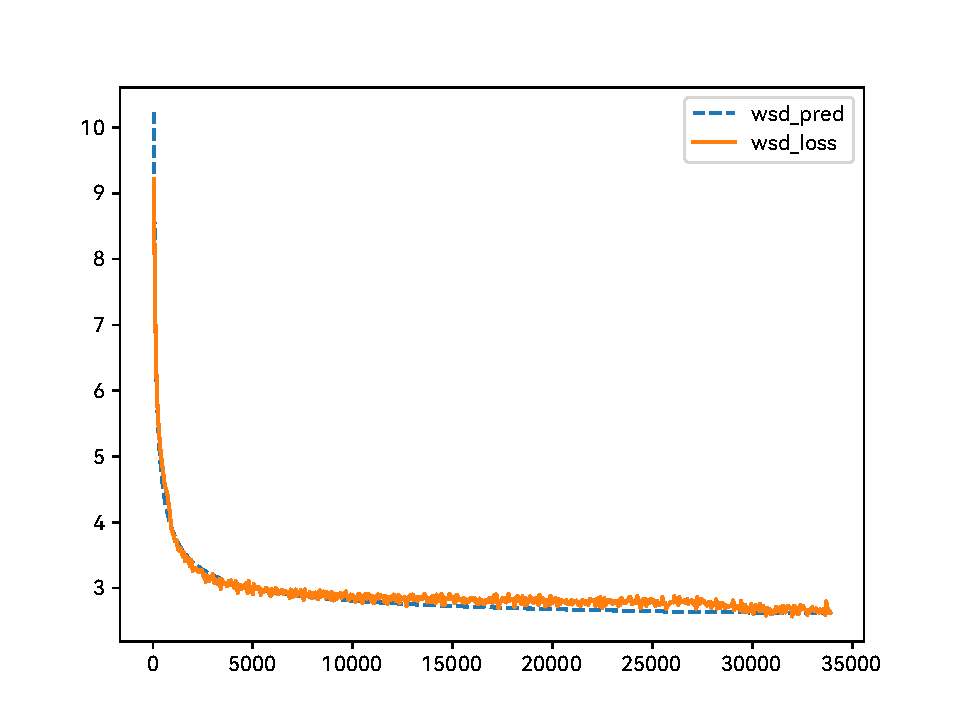
\includegraphics[width=0.3\textwidth]{fig/lra/wsd_fit.pdf}
            }\label{fig:figure}
        \end{figure}
    \end{frame}

    \begin{frame}
        \frametitle{Experiments Results of MPL}
        We use cosine learning rate schedule to fit the parameters
        \begin{figure}
            \centering
            \subfigure[cosine learning rate]{
                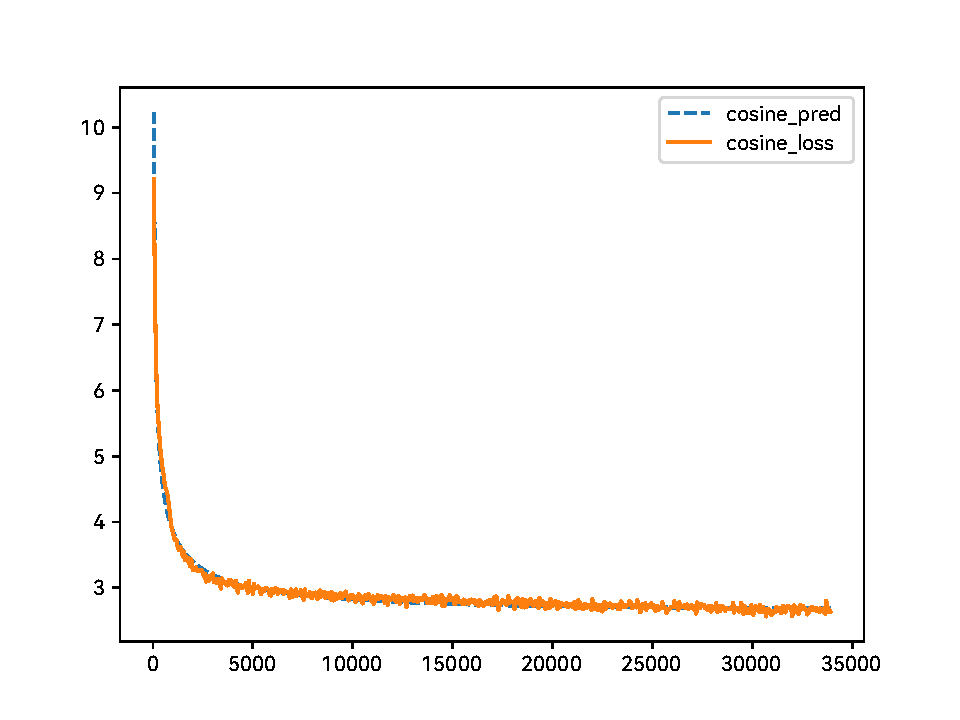
\includegraphics[width=0.3\textwidth]{fig/mpl/cosine_fit.pdf}
            }
            \subfigure[8-1-1 learning rate]{
                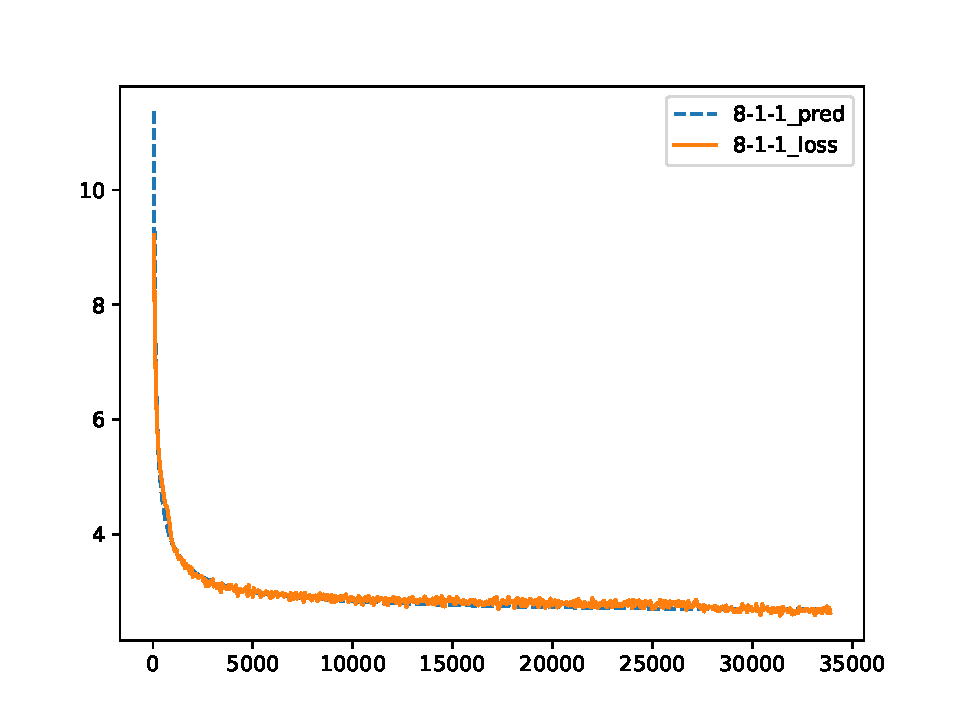
\includegraphics[width=0.3\textwidth]{fig/mpl/8-1-1_fit.pdf}
            }
            \subfigure[WSD learning rate]{
                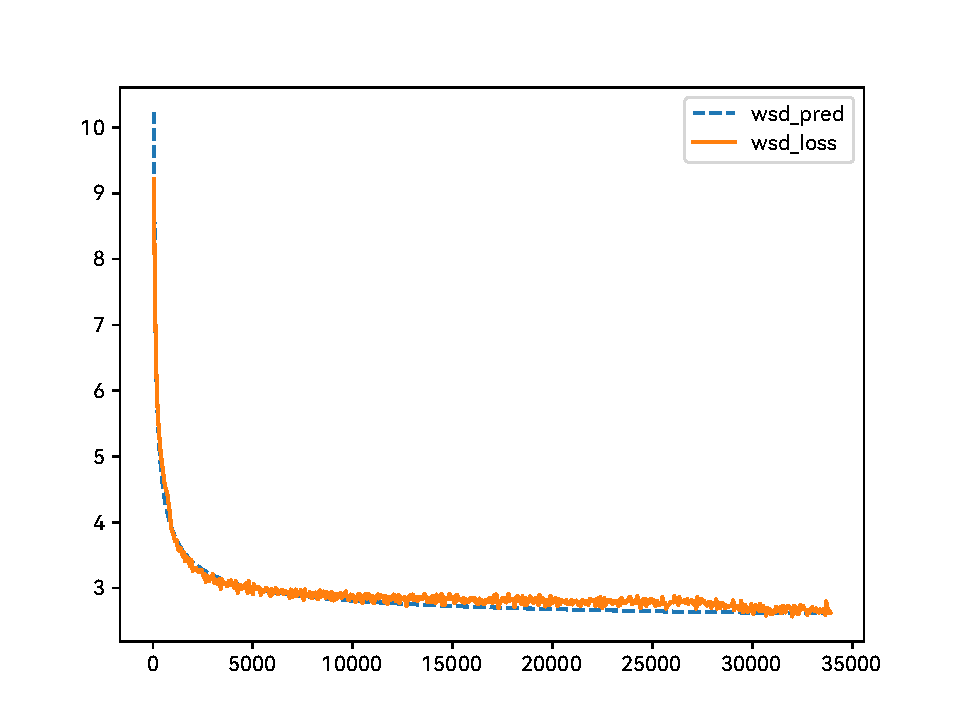
\includegraphics[width=0.3\textwidth]{fig/mpl/wsd_fit.pdf}
            }\label{fig:figure2}
        \end{figure}
    \end{frame}

    \begin{frame}
        \frametitle{Error of Fitting}

        The table below shows the fitting errors (MSE) of different scaling laws.
        \begin{table}[htbp]
            \centering
            \begin{tabular}{lcccc}
                \toprule
                Scaling Law & Schedule for Train & Cosine & 8-1-1
                & WSD \\
                \midrule
                LRA & Cosine & 4.4769e-02 &
                5.7181e-02 & 5.7885e-02 \\
                LRA & 8-1-1 & 4.5892e-02 &
                5.6336e-02 & 5.7780e-02 \\
                LRA & WSD & 4.4450e-02 &
                5.2244e-02 & 5.3246e-02 \\
                MPL & Cosine & 5.1094e-02 &
                6.1200e-02 & 5.9661e-02 \\
                MPL & 8-1-1 & 5.7103e-02 &
                5.5278e-02 & 5.3867e-02 \\
                MPL & WSD & 6.1385e-02 &
                5.2909e-02 & 5.1991e-02 \\
                OPL & Cosine & 5.1286e-02 &
                6.1284e-02 & 5.9737e-02 \\
                LLDL & Cosine & 5.1094e-02 &
                6.1200e-02 & 5.9661e-02 \\
                MEL & Cosine & 5.1115e-02 &
                6.1220e-02 & 5.9674e-02 \\
                \bottomrule
            \end{tabular}
            \caption{Fitting errors of different scaling laws}
            \label{tab:fitting_error}
        \end{table}

    \end{frame}

    \begin{frame}
        \frametitle{Phenomenon and Analysis}
        \begin{enumerate}
            \item[1] As shown in Table \ref{tab:fitting_error}, the
            fitting errors of all scaling laws under different
            training-test splits show minimal variation and remain
            below 0.1. This indicates that all scaling laws are
            effective in this set of experiments.
            \item[2] In the ablation experiments, we observe that
            modifications to the $LD(t)$ component result in
            negligible changes to fitting errors.
            This occurs because the learning rates in our
            experimental data vary smoothly, making this term several
            orders of magnitude smaller than the $S_1$ term, thereby
            exerting limited influence on the fitting outcomes.
        \end{enumerate}
    \end{frame}

    \begin{frame}
        \frametitle{Phenomenon and Analysis}
        \begin{enumerate}
            \item[3] Due to the minimal influence of the $LD(t)$ term,
            fitting curve of MPL closely approximates a simple power function.
            In contrast, fitting curve of LRA better captures the
            nuanced variations in loss (as illustrated in the figure
            below), thereby demonstrating superior fitting precision.
        \end{enumerate}
        \begin{figure}
            \centering

            \subfigure[LRA]{
                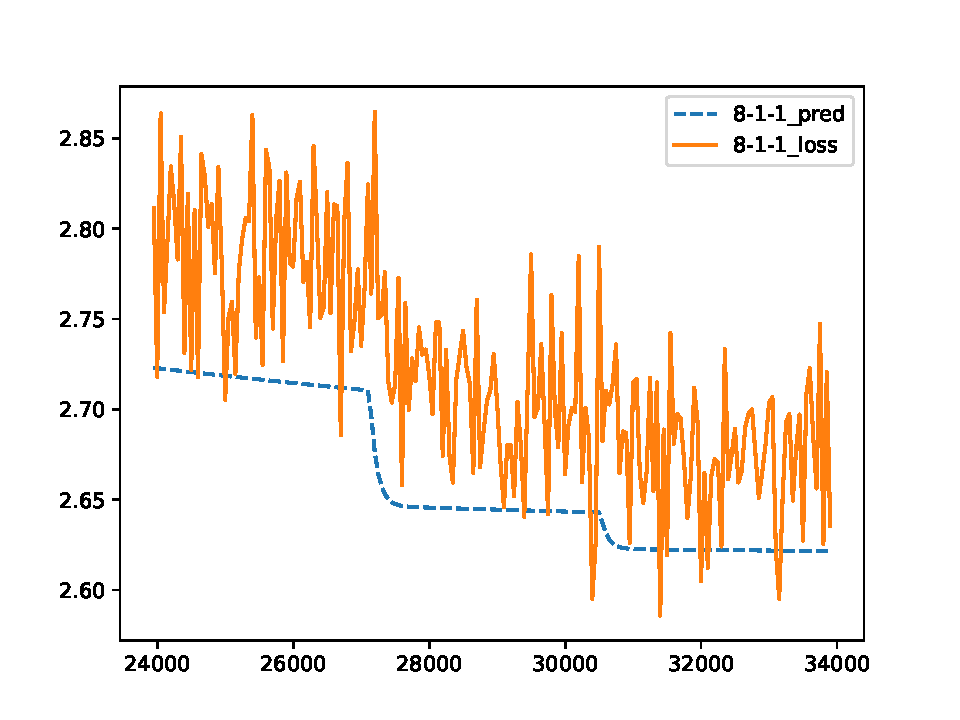
\includegraphics[width=0.4\textwidth]{fig/comparison/8-1-1_LRA}
            }
            \subfigure[MPL]{
                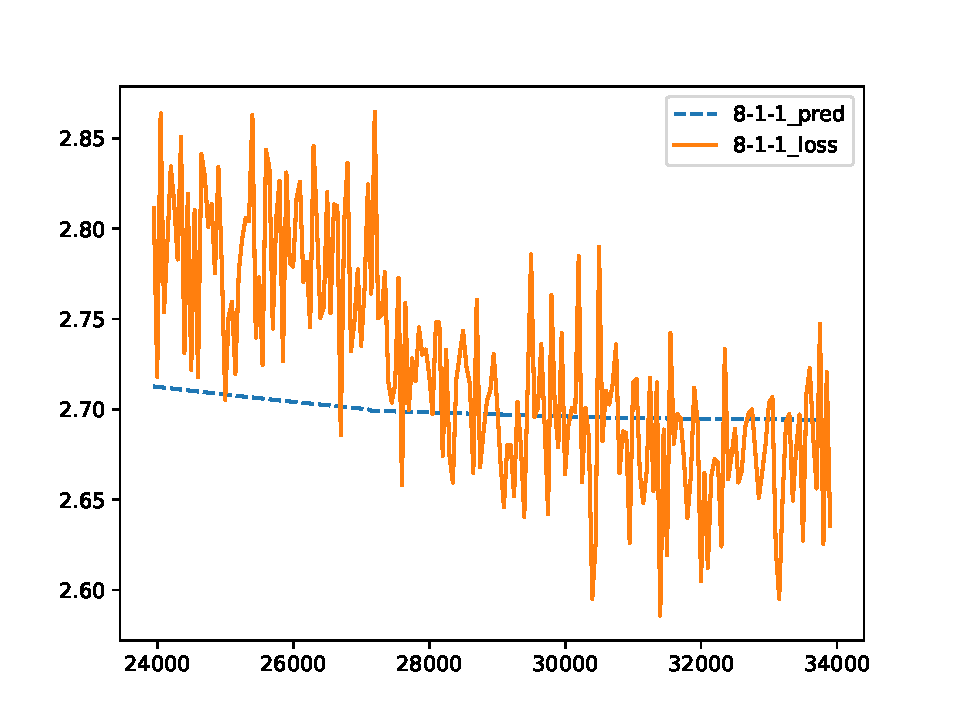
\includegraphics[width=0.4\textwidth]{fig/comparison/8-1-1_MPL}
            }
            \caption{Comparison of LRA and MPL fitting curves}\label{fig:figure3}
        \end{figure}
    \end{frame}

    \begin{frame}
        \frametitle{Optimal Learning Rate Schedule}
        Using MPL\eqref{eq:multi_power_law},we parameterize the predicted
        final loss as $\mathcal{L}_\Theta(E)$ with parameters $\Theta =
            {L_0,A,B,C,\alpha,\beta,\gamma}$ to get a optimization problem:
        $$
        \min_E \mathcal{L}_\Theta(E) \ \ s.t.
        \ \ 0\le\eta_t\le\eta_{t-1}, \ \forall t\in[1,T]
        $$
        Solving this problem,we can get the optimal learning rate
        schedule plotted in the figure below.
        \begin{figure}
            \centering
            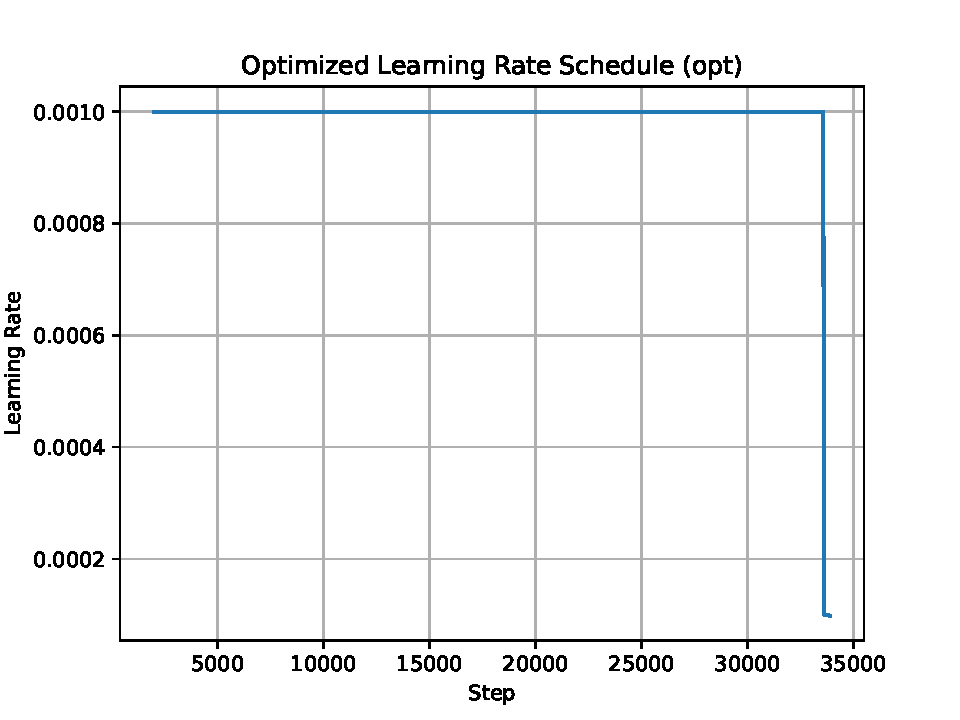
\includegraphics[width=0.35\textwidth]{fig/opt/opt.pdf}
        \end{figure}

    \end{frame}


    \section{Simple Power Law}\label{sec:simplepowerlaw}

    \begin{frame}
        \frametitle{Discussion on Multi Power Law}
        Our group did not use the code provided by the original authors, but instead independently implemented the algorithm described in the paper.
        During our experiments, we observed that the parameters $B$, $C$, $\beta$, and $\gamma$ exhibited almost no variation throughout training. To investigate their actual impact, we performed a series of empirical evaluations.

        Our experiments revealed that manually setting a large value for $B$ allows the resulting model to fit the trend of the loss curve quite well. However, $C$ appeared to have virtually no effect during the experiments. The parameters $\beta$ and $\gamma$ only had an impact within certain ranges, and even then, their influence on the results was marginal.

        Moreover, although a larger $B$ helps the curve better track the loss trend visually, due to a shift in the mean, it does not necessarily lead to improved metrics such as MSE or $R^2$. This further confirms that the gradient with respect to $B$ is indeed very close to zero.

        In fact, the code provided by the paper’s authors is also unable to effectively optimize the parameter $B$. Their implementation selects $B$ from a set of hardcoded ``magic numbers'' rather than optimizing it in the conventional sense.
    \end{frame}
    \begin{frame}
        \frametitle{Discussion on Multi Power Law}
        %TODO: add figures
    \end{frame}
    \begin{frame}
        \frametitle{Simple Power Law}
        In practice, simply setting $G(x) \equiv 1$ in MPL and assigning $B$ as a predefined parameter can already produce a good fit to the loss trend—and in some cases even achieve better results in terms of MSE. We refer to this approach as the \textbf{Simple Power Law (SPL)}, which suggests that the trend of training loss in large models is, in a loose sense, proportional to the change in learning rate.
    \end{frame}

% THANK FOR YOUR ATTENTION
    \begin{frame}
        \frametitle{}
        \begin{center}
            \Huge Thank You for Your Attention!
        \end{center}
    \end{frame}

\end{document}